\renewcommand\labelenumi{(\roman{enumi})}
\renewcommand\theenumi\labelenumi

\chapter{Introduction}
\label{chapterIntro}
\chaptermark{Introduction}

The current society is facing a challenge in order to mitigate the effects of the climate change. With the objective of keeping global temperature rise below 2 degrees Celsius as stated in the Paris Agreement XXXX, the whole energy system is called to an action: transform a mainly fossil-based electricity generation scenario to one that is carbon-neutral, mainly based on renewables energy sources (RES). The challenge is even greater, since it is expected that the electricity consumption will increase from a 20\% to 40\% by 2050, according to \cite{IRENA2018}. This can be observed in Figure \ref{fig:scenarios}, where the scenario by 2050 expects the 85\% of the electricity supply to be covered by renewables. 

\begin{figure}[]
	\centering 
	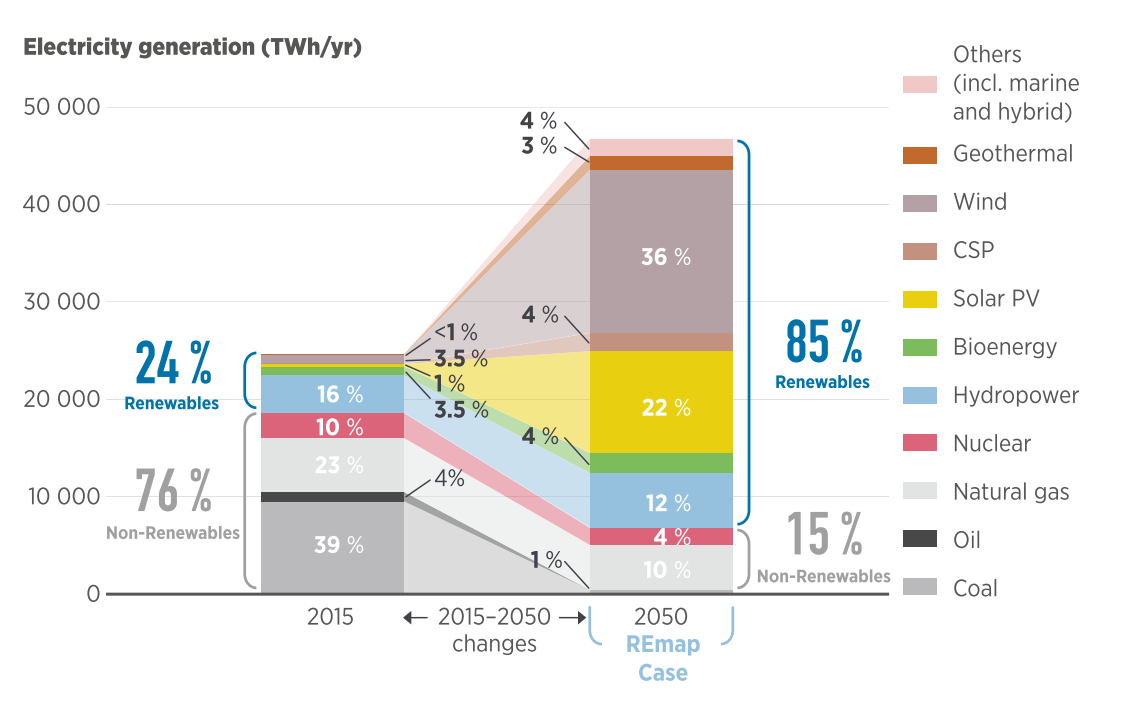
\includegraphics[width=1\columnwidth ]{ChapterIntro/Figures/irena_scenarios.png}
	   %\vspace*{-8cm}
		\caption{Renewable Energy Sources penetration scenario. Extracted from \cite{IRENA2018}}  
		\label{fig:scenarios}
\end{figure}

Despite the scenarios where renewables are the main source for electricity production, it is a fact that large power plants placements are more difficult to find XXX, leading to newer technologies to allocate renewable sources in places where a larger power output can be obtained, and less concern by end-users in terms of environmental and visual impact of them, such as off-shore wind turbines XXXX, connected to the transmission network. At the same time, as electricity demand on grids increased due to the electrification of appliances, distribution system operators (DSOs) started to face congestions in their networks, and hence utilities started to find solutions for managing these peak loads, usually located in specific time periods.  This combined to the implementation of smart meters so utilities could encourage customers to switch consumption from peak to non-peak hours, and the need for monitoring and controlling the operation of the distribution network enhanced the development of smart grids. Traditionally, electric power system have been centralizsed structures organized into generation, transmission and distribution, placing end-users and the endpoint of the supply chain. This was an unidirectional structure where electricity generated by large power plants was transported by means of transmission and distribution networks, to be delivered to end-users. Despite, the emergence of the social awareness of the environmental impact of the end-users consumption, the increase of the electricity prices, as well as the emergence of the so-called distributed energy resources (DERs), such as small-scale PV installations (mainly rooftop), storage systems, electric vehicles (EVs) and smart home appliances are transforming the end-users into active participants in the power system. The increasing penetration of these decentralized resources, as well as the emergence of new market agents like prosumers, aggregators and active consumers, are pushing the electricity system to include innovation in their business models, creating the paradigm of smart grids. 
According to \cite{EuropeanParliamentSG}, smart grids can be defined as an electricity network that can integrate in a cost efficient manner the behaviour and actions of all users connected to it, including generators, consumers and those that both generate and consume, in order to ensure an economically efficient and sustainable power system with low losses and high levels of quality, security of supply and safety. 
However, it it nos only in terms of technological innovation to fulfill the electricity transition roadmap. Changing the regulatory framework mainly for DSOs to adapt the current regulation for the operation of the distribution network to the new challenges placed by DERs is a key factor for the success of the energy transition. 
This chapter aims to provide an overview of the current state of the electricity system and their agents, so as to highlight the main shortcomings, challenges and opportunities for the implementation of the energy transition roadmap. The following pages cover the regulation related to DSOs and smart grids, the technical aspects of DERs and ICT technologies, the role of demand-side and end-user's awareness, and lastly the role of new business agents and services that can help DSOs to become key agents in the development of smart grids. 
INTRODUCE NEW FIGURE 
\begin{figure}[]
	\centering 
	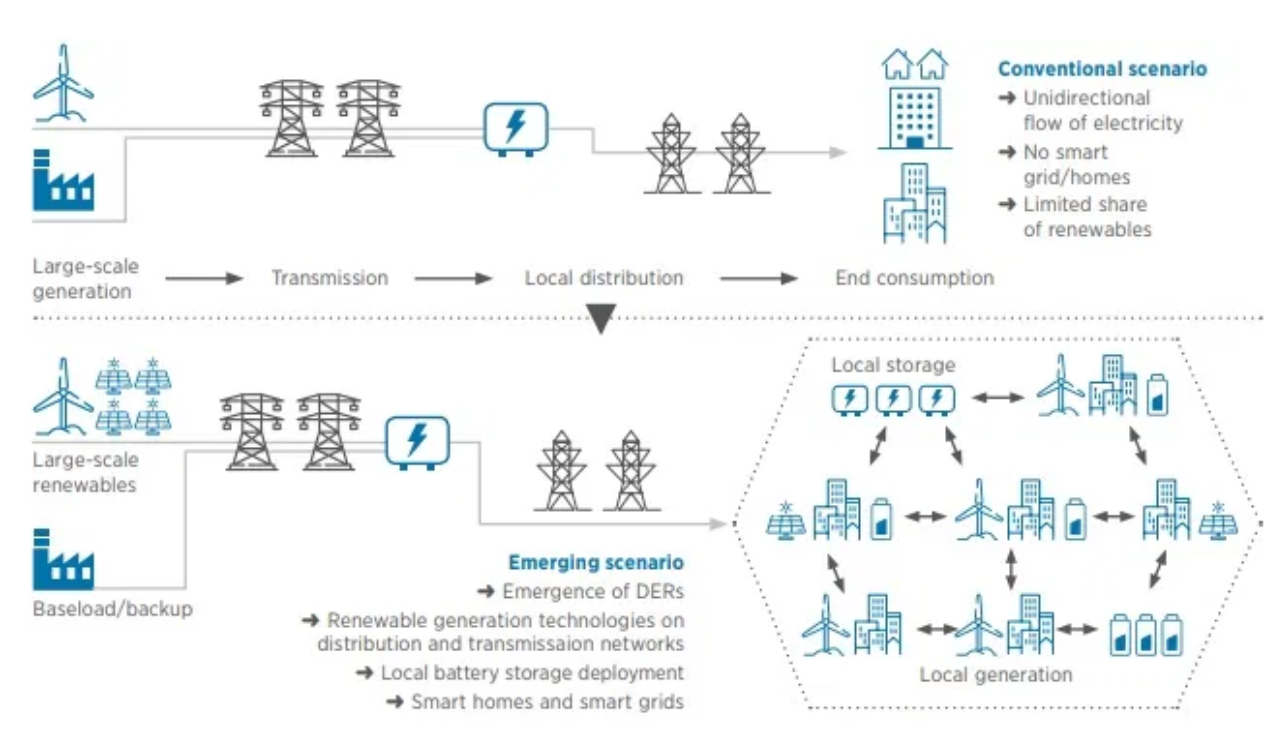
\includegraphics[width=1\columnwidth ]{ChapterIntro/Figures/Irena-DSO-1.png}
	   %\vspace*{-8cm}
		\caption{Conventional scenario. Extracted from \cite{IRENA2018}}  
		\label{fig:scenarios}
\end{figure}

%Explicar el problema al qual ens estem adre\c{c}ant 

%\textcolor{red}{20-25 PAGINES}

%\textcolor{red}{Fer a la intro, despres de quan introdueixo els local markets icons,m quan he dexplicar la contribucio a la tesi. Explicar quin son els tres agents que analitzo, en aquest cas dos, aggregator i DSO. I llavors posar la interaccio entre ells, la flex request, flex forecast i flex activation, posar tots els agents. Llavors a cada chapter indico quina cadena estic treballant, i despres en difuminat indico quina cadena no estic activant.}
%
%\begin{figure}[]
%	\centering
%	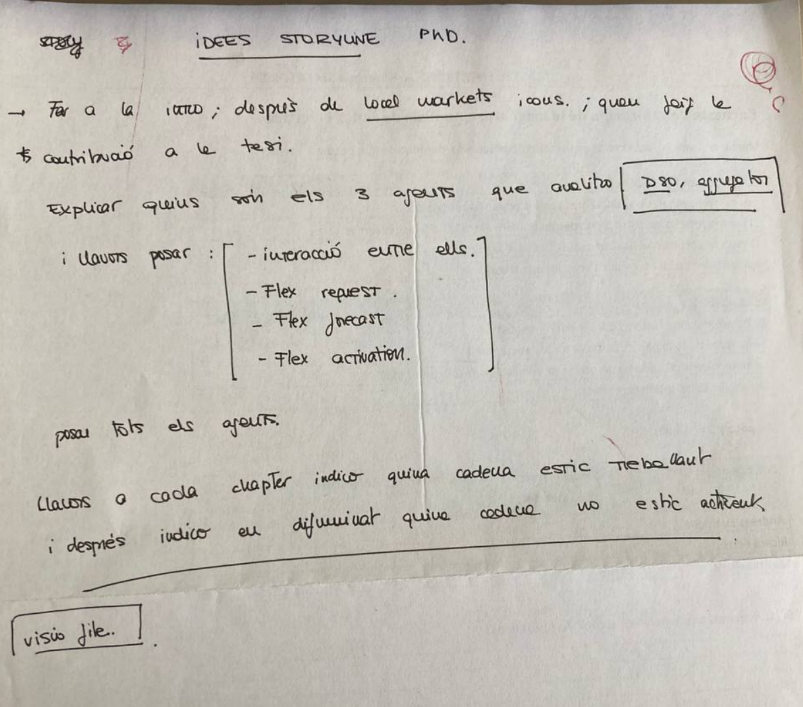
\includegraphics[width=1\columnwidth ]{ChapterIntro/Figures/idea.png}
%	   %\vspace*{-8cm}
%		\caption{XXXX}  
%\end{figure}

%\section{Smart grids}
%
%\subsection{Distributed Energy Resources} \label{subsec:DG}
%
%\section{Distribution networks: challenges}
%
%\section{Electricity markets}


\section{Regulation framework and new agents in the energy transition}

The following pages cover the regulation related to DSOs and smart grids, the technical aspects of DERs and ICT technologies, the role of demand-side and end-user's awareness, and lastly the role of new business agents and services that can help DSOs to become key agents in the development of smart grids. 



\section{Smart Grids related technologies: ICTs and }

\section{Sustainability of smart grids and DERs}
Explicacio sobre que entenem per sostenibilitat. Quina relacio hi ha entre sostenibilitat i smart grids local markets 

\textcolor{red}{Incloure la part de rebuig a les renovables, de que no hi ha espai per a grans emplacaments i que per tant la solucio passa per generacio local i demand side management}


\newpage 
\section{Objectives and scope}
Several past and recent works in the literature have dealt with the development of smart grids and defining local electricity markets for enhancing the energy transition. The majority of these studies consider flexibility as a known signal, assuming a perfect forecast and a direct control of the flexible assets, as a way of simplifying the operation of the local flexibility markets. Furthermore, they assume that both the aggregator and the DSO share information regarding the flexible assets or the network layout. The fact is that, in reality, and according to the current regulation, they must be different entities, considering 

The main research question that this thesis aims to answer is the following one:

\begin{tcolorbox}
What are the possibilities to develop and activate flexibility in distribution networks, by engaging demand-side and ensuring that the sustainability goals are taken into consideration? 
\end{tcolorbox}

\textcolor{red}{Explicar una mica quina son les opcions que veiem}

Based on the previous discussion, more specific objectives can be outlined in order to set the basis for the research developed in this thesis. The objective of the thesis are outlined below: 

\begin{tcolorbox}
\begin{enumerate}
\item What are the possible market schemes to integrate DERs and demand-side management, while at the same time ensuring that network operators can benefit from these services?  
\item How can flexibility be defined and modeled, based on the final users providing and using this flexibility, as well as the time horizon purposes? 
\item How can flexibility be forecast, from the aggregator point of view, with very limited amount of data available, in a fast and reliable approach so as to know in advance the flexibility available in the portfolio, in order to provide flexibility to DSOs for operation purposes?
\item How can this flexibility help DSOs to mitigate or avoid congestions in MV networks, and how can this flexibility request be calculated so as to be economically better than investing in network expansion or hosting capacity?
\item How this scenario of flexibility provision can be environmentally assessed, so as to know if these approaches can be included in each and every country? Should the current installed capacity and generation portfolio be taken into account before the deployment of flexibility services in smart grids?
\end{enumerate}
\end{tcolorbox}


\begin{figure}[]
	\centering 
	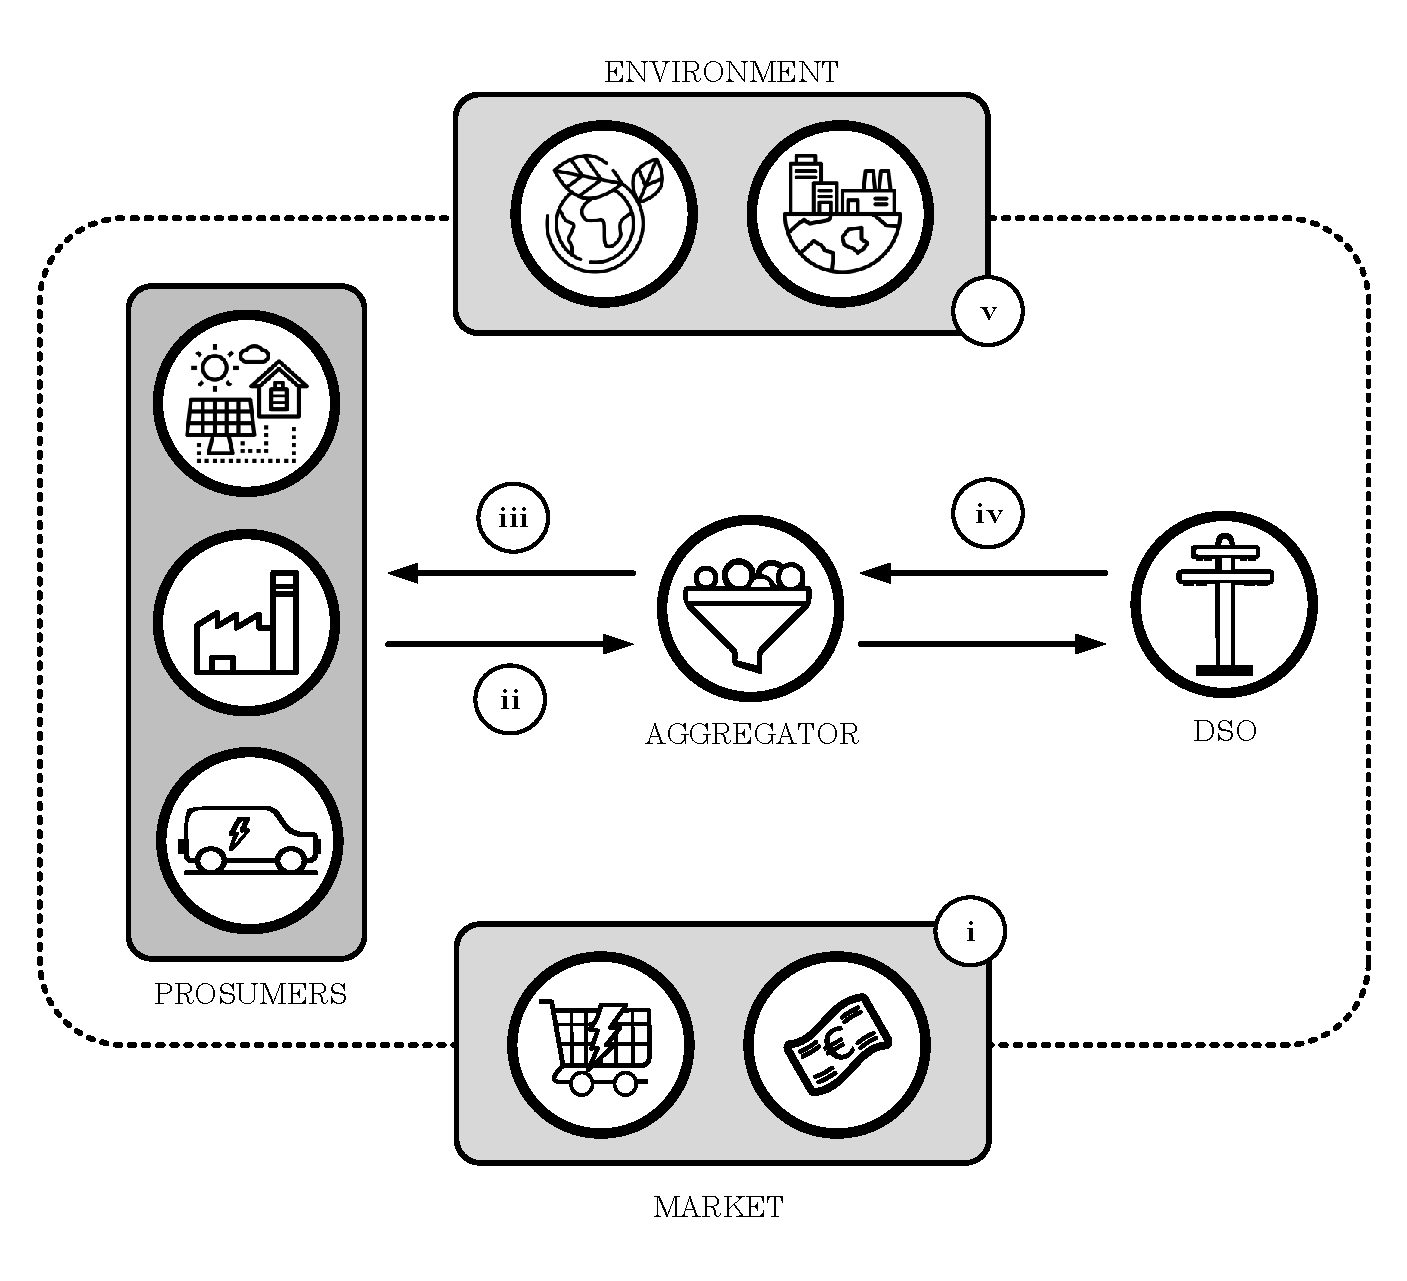
\includegraphics[width=0.9\columnwidth ]{ChapterIntro/Figures/objectives_figure_2.pdf}
	   %\vspace*{-8cm}
		\caption{Overview of the thesis objectives}  
		\label{fig:objectives}
\end{figure}


\newpage 
\section{Thesis related work and activities}
This section provides a summary of the work and the relevant activities that the author has participated in during the developlment of the thesis presented in this manuscpript. 
 	
Doctoral activities started in June 2017 with the collaboration on behalf of the EMPOWER \textit{Local electricity retail markets for prosumer smart grid power services } Project (Grant Agreement No. 646476). This work consisted on a review of the current state of the art in terms of Life Cycle Assessment Methodology in the field of smart grids, the understanding of how this methodology can be implemented in power systems and renewable energy technologies and the assessment of the environmental impact of the pilot-sites implemented throughout the project. This research resulted in a presentation in the General Assembly of the H2020 Project [P-C1] and the technical report [TR-2]. The research on the environmental assessment of ICT and Smart grids continued in the H2020 Project INVADE \textit{Integrated electric vehicles and batteries to empower distributed and centralised storage in distribution grids} (Grant Agreement No. 731148), in years  2018 and 2019, with the assessment of the environmental impact of electricity generation and the possibility of including flexibility to lower the environmental impact of electricity production in the INVADE pilot-sites. This research was performed in collaboration with the Finnish research center VTT, NTNU, Elaad and eSmart resulted in the journal publication [J1], a conference proceeding [C2], and technical reports [TR3], [TR5]. Dissemination events for the exploitation of the results took place in years 2019 and 2020, [P-C5] and [P-C11]. 

Since the main objective of the thesis is how new local markets and new service can help the deployment of smart grids, a thorough review of the state-of-the-art on local electricity market was done as a starting point of the doctoral research in 2018. This research was mainly focused on describing the basics on power systems and market mechanisms, as well as a literature review on local and micro-markets. As a result of that, a technical report was developed [TR1], and two book chapters were published by Wiley ([BC1],[BC2]).  The evolution of this state-of-the-art review, combined with the collaboration with colleagues at CITCEA-UPC and other research centers and companies such as EYPESA and Smart Innovation Norway or on behalf the INVADE Project led to several outcomes covering from technical reports [TR4], journal articles [J4] adnd [J5]; conference papers [C1], [C3] and [C4]; and presentations in local and international events [P-C3] and [P-C4].  

The evolution and implementation of smart grids based on data-driven approaches has been of interest of the author, and combined with collaboration with other universities as KU Leuven, DTU and KTH Stockholm on behalf of EIT InnoEnergy, resulted in [P-C6], [P-C10] and [P-C14]. 

%Escriure BD4OPEM aquí 
Year 2020 started with the kick-off the BD4OPEM H2020 Project \textit{Big Data for Open Innovation Energy Marketplace} (Grant Agreement No. 872525), with the participation of 12 partners from 8 different countries, and 5 pilot-sites. The research consisted on the development of algorithms for flexibility forecast and distribution network congestion management based on optimization techniques and flexibility provision. This work was combined with the Technical University of Denmark (DTU) under the external stay of the author, and in collaboration with other research centers and companies such as JSI and ICOM. This work resulted in a technical report [TR6], two dissemination events [PC-12], [PC-15], and three journal publications under review or preparation [J2], [J3] and [J6].  

The international placement took place from March 2020 until April 2021, at the Electricity Markets (ELMA), DTU, Kongens Lyngby, Denmark. The topic was aggregated flexibility forecast based on probabilistic forecast techniques. It resulted in a journal paper [J2], and the database publication [DB1]. During this period, the author has collaborated with KU Leuven in the core of the Data Science Working Group, with the aim of improving the knowledge of undergraduate students in the field of data science in the energy sector. This resulted in the publications [J7] and [J8]. 

Since the author and the research center where the thesis was involved has a flair for knowledge transfer and higher and professional education, the author has collaborated with other entities and other researchers, resulting in the respective outcomes, which are not included in the thesis manuscript. This is the case of the collaboration with EIT InnoEnergy. This European institution has as a main core activity the connection and collaboration between industry, universities and research centers with the objective of reducing the gap betwen research and the market. In years 2018, 2019 and 2020 the author has been the lead teacher of the course on Control and Automation for the Efficient Use of Energy, developing the open-source learning material and developing a course based on project-based learning and flipped classroom approach. This resulted in several activities, such as [E1] being the learning material, and dissemination of the results in different local conferences [P-C2], [P-C7] and [P-C8]. The project Learning Analytics started in September 2018, with the objective of monitoring students' performance to assess their engagement in the course, in collaboration with the Data Collection company DataLemon. This collaboration led to dissemination event [P-C9] and [P-C13], as well as an ongoing journal paper to be submitted in the near future. Other collaborations within the Electrical Engineering Department led to two outcomes: a MOOC courses for wearable technology [E2], and a publication in a local journal [C5]. 


\newpage 
\section{Thesis outline}
The content of the thesis is organized in the following chapters as follows:
\begin{itemize}
\item \textbf{Chapter 2} presents the overall state-of-the-art in terms of local energy markets, in order to define the role of flexibility in a local market and to which extent this service can help energy transition, and more specifically, DSOs. This work correspond to the first objective of the thesis \textit{(i)}. 
\item \textbf{Chapter 3} outlines how flexibility can be formulated, defined and modelled according to different approaches in terms of end-user, approach and time-horizon, covering the second objective of the thesis, providing different formulations for modeling flexibility \textit{(ii)}. 
\item \textbf{Chapter 4} presents the aggregated flexibility forecast for estimating the available flexibility within an aggregator's portfolio, with limited amount of information, for operation purposes and trading in a market or a bilateral contract. This chapter aims to fulfill the thirds approach of the thesis \textit{(iii)}. This formulation is implemented under a case study covering a portfolio of flexible assets such as Electric Vehicles, Space heaters and electric water boilers.  
\item \textbf{Chapter 5} outlines the AC-OPF formulation for calculating the flexibility requests needed by DSOs to solve congestions in MV networks by means of flexibility activation. This chapter corresponds to the fourth objective of the thesis research \textit{(iv)}.  
\item \textbf{Chapter 6} extends the scope of the previous research assessing the potential role of flexibility in different countries, in terms of sustainability. This chapter calculates the peak-hour environmental impact measured in $CO_2$ emissions, so as to establish a baseline for countries to understand where DERs and flexibility could be implemented and leading to a lower carbon footprint. This chapter focuses on the last objective of the research \textit{(v)}. 
\item \textbf{Appendix A} enumerates the publication and research outcomes both related and non-related to the thesis manuscript. 
\end{itemize}


